\section{Introduction}
For digitization projects, the construction industry is yet a mostly unconquered field.
Complex dynamics and sometimes harsh (e.g. weather influence, no infrastructure, etc.) environments of construction sites challenge the technology and adds harder requirements compared to an industrial application on a shop floor. 
Moreover, the typically conservative and hierarchical work culture makes the introduction and acceptance of new methods more challenging. In this paper, we describe the vision and ideas behind the ConWearDi project and its approach to better understand and overcome these challenges.

\section{Project scope}
Construction projects vary highly in size and complexity from huge civil engineering projects to building a small house. 
The ConWearDi project focuses its efforts on improving efficiency of smaller constructions, e.g. interior work, painting of houses, and craftsman businesses.
Challenges included for such business are different than those a big multinational corporation with thousands of workers has to face, but nonetheless very interesting and important.

\section{Problem description}
The construction industry shows huge potential for digitization and is still in the early phase of adopting technologies related to Industry 4.0. 
While Building Information Modeling (BIM) is used more frequently for processes of the design and planning phase, the actual construction and execution process of the value creation, is still dominated by analog processes and paper documents. 
Examples include wall sized printed plans and time sheets on paper, which are adjusted with delay and only digitally recorded in offices, only available there. 
So, in many cases, the digital world ends in the back office or at the workstations of the architects, managers and foremen. 
The potential of novel services, such as Internet of Things (IoT) systems with sensors and actuators deployed on site connecting it to powerful computing resources, remained untapped.

\section{Project goal}
The goal of the ConWearDi project is the design and prototype implementation of a platform capable to capture and analyze the current state of construction work and to provide useful informational support not only for the managers and architects but directly to the construction workers and craftsmen on site. 

%Information sources, which provide structured information and accurate specifications (e.g. used materials) about a project, such as the BIM itself, are the foundation to achieve this goal. These

The main project goals can be summarized as:
\begin{enumerate}
  \item Creation of a Digital Twin, a representation of the construction site, which always reflects its current state 
  \item Centralized system for managing the construction site
  \item Automatic documentation for knowledge- and quality management purposes
  \item Exploration of new business models
  \item Development of methods for monitoring the activities of different worker groups with wearable technologies
\end{enumerate}

\section{Vision}

\begin{figure*}[htp]
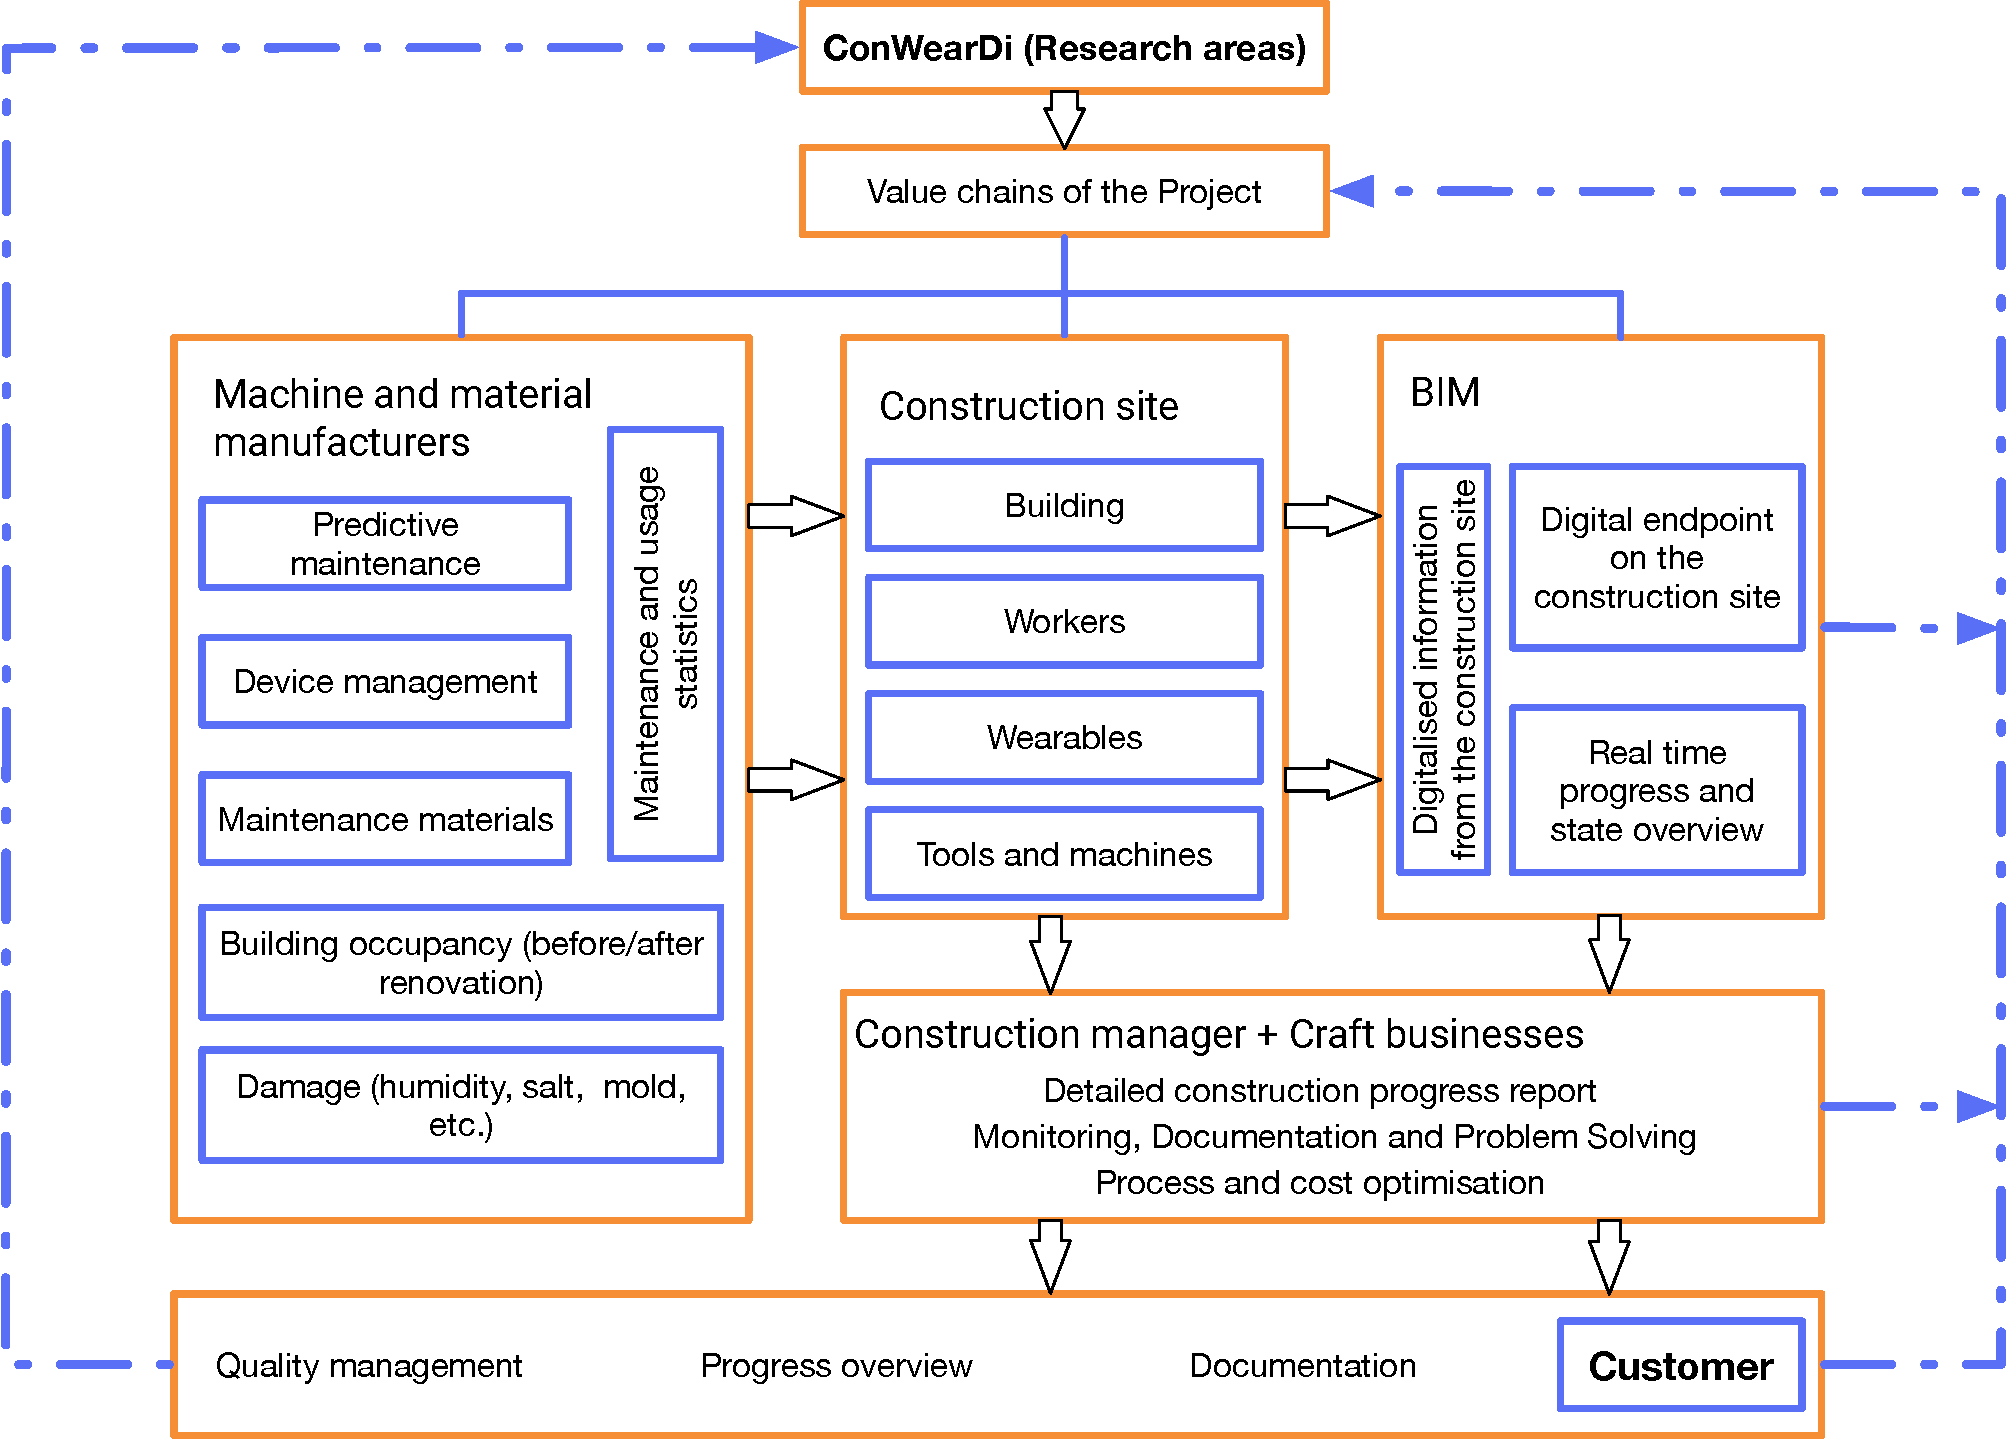
\includegraphics[width=0.8\textwidth]{figures/conweardi-functional.pdf}
\caption{Functional graph}
\label{fig:functional}
\end{figure*}

The most significant benefit, we envision through realization of the ConWearDi system, is better efficiency in detecting and preventing problems and damages by improving or if possible fully automatizing construction site documentation and reporting workflows. 
Utilizing a real time information flow from the construction site, planners and managers are able to anticipate upcoming issues and avoid costly delays and damage repairs. 
Communication between customers, managers, designers and workers will also be improved by bundling of information such as agreements, used materials, tools and recorded working hours.
All in all, every stakeholder in the construction process will benefit from such a system. 
In the following paragraphs, we describe what new or improved services each participant of the process would be able to use during the execution of their role.


\subsection{Construction site manager}
Similar to industrial control processes, the construction site's current state would be available real time through its digital twin.
This could help to recognize and avoid execution problems, e.g. when storage levels of the required materials are running low.
Auto-generated reports unload this time consuming task from the construction manager, and allow a more detailed documentation over time, saving the full history of the building creation.
This has major impact in later phases of construction or even in other phases of the building's life cycle, when previous decisions can be retraced and interface problems can be recognized. 

Continuous monitoring is also a powerful tool for the construction manager to fulfill his responsibilities about work safety and protecting the employees health. In a simple example, this can mean to prevent health risks caused by overtime or using heavy machinery without breaks and longer than allowed.
The accumulated knowledge can be used in other projects by learning from previous experiences (e.g. objective analysis of what went well, what went wrong).

\subsection{Designer and project coordinator}
Coordination processes can rely on digitally documented commitments instead of verbal agreements, since they are just as simple to create.
The project coordinator also benefits from the simplified, IT-supported trade-coordination based on the methods of Advanced Planning and Scheduling (APS).
Automatic documentation processes can be easily adapted later to support new standards and regulations, e.g. for fire safety.
The high resolution data can be fed into big data analytics services, e.g. to detect patterns across multiple construction projects which allows new possibilities to improve organizational processes.

\subsection{Machine and tool manufacturers, material suppliers}
For machine, tool and material producers and suppliers, the increased connectivity of their devices and their integration into the digital processes of their customers helps to better understand the market and customer behaviors. 
Based on the collected information, they can implement more efficient service and logistic coordination e.g. by predicting when will be the customer's material storage depleted.

They can offer a proactive maintenance service for construction site machines based on their usage and wear tracking. 
Furthermore, machine manufactures can adapt new business models which rely on the connectivity and the sensors of their machines. An example is the just in time machine leasing, where customers pay only for the time when they really used the machine.

Material suppliers can offer proactive maintenance services for built-in materials by tracking their physical state and properties (e.g. temperature and humidity).
With the ever growing amount of collected sensor data and customer feedback, they can develop and test new solutions for the market.


\subsection{Craftsman businesses and construction workers}
For craftsmen and workers on the field, the system provides the possibility to access context related, reliable and up-to-date information easily. 
This can improve also help to ensure execution quality and the work safety by preventing mistakes caused by miscommunication.
For the organization, this usually means less phone calls and traceable information flow.

By using connected devices, the manufactures can offer real time remote support services to help the workers on site to solve problems and reducing costly down-times waiting for a replacement machine or a technician.
The system gives the workers to easily report disruptions in the processes, which with careful analysis could help the organization on the way of continuous improvement.

The real time target-performance measurements allow to avoid foreseeable delays with simulating and providing alternative solutions. This leads to a generally optimized resource usage and a smart decision support system.


\section{Methodology}
The realization of the above described vision is a complex task, even if many of the necessary systems exists and are used in other industries. 
They have to be adapted to the particular requirements and work culture of the construction industry. 
The approach of the ConWearDi project for solving this task is to include experts from different profession and many possible stakeholder for the proposed system.
 
Figure \ref{fig:functional} shows the functional structure and main value chains of the ConWearDi project. 
The actual research question are oriented on the most important factors for the end customer. 
These topics are then projected into the main value chains, e.g. how can the machine manufacturer contribute to the success and efficiency of the construction project and so on. 




\section{Conclusion}
\todo{high potential to digization - still many unsolved problems - project is focusing to making first demonstrators - running at first real businesses}

\todo{for more information visit project website}

\begin{acks}
  This work has been funded by the Federal Ministry of Education and Research of Germany (BMBF) within the framework of the project ConWearDi.
\end{acks}
